\section{Code Generation}
\label{sec:code_gen}

In this section, we discuss the compiler passes used to construct BBE program
binary as well as the micro-architectural blocks designed to support BBE.

We run binary translation on the x86 ISA to generate the program control flow.
Once basic-blocks are identified, a number of elements in each BB must be set;
special basic-block header (\texttt{Head}) instructions must be inserted, an
energy-aware register allocation model is run, and instruction scheduling is
done to generate the optimal static schedule for each basic-block.  In this
work, a basic-block is defined to end with a \texttt{br}, \texttt{jmp},
    \texttt{call}, or \texttt{return}. It is also terminated when the the
    basic-block reaches 16 instructions. %TODO specify how rare is this

\begin{figure}
	\centering
	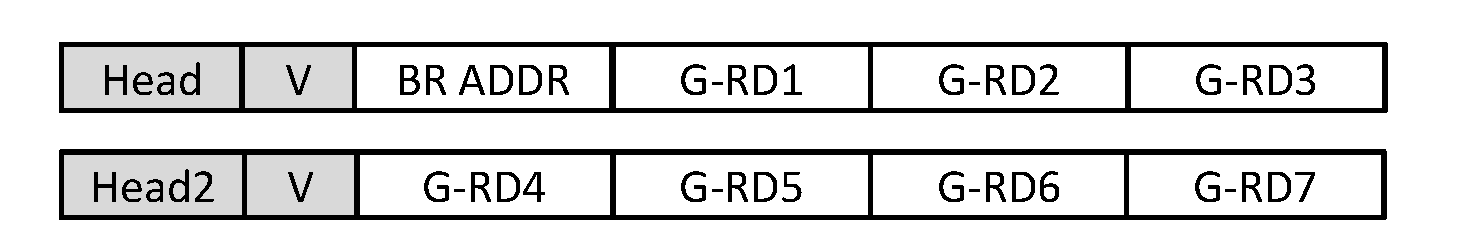
\includegraphics[width=1.0\columnwidth]{fig/header_ins.pdf} 
    \caption{\texttt{Head} and \texttt{Head2} instructions represent BB
        header information. \texttt{Head2} is only used for basic-blocks with
            more than three global read operands. BR ADDR represents the address
            offset of the branch operation at the end of the BB. V bits specify
            how many of the register operands are valid and whether BR ADDR
            holds a valid entry.}
	\label{fig:header_ins}
\end{figure}

Two register allocation passes are done on the compiler to generate instruction
operands. The first pass finds the register operands live beyond the boundaries
of the basic-block, and the second pass allocates registers live only within the
basic-block boundaries. The former is a global register and the latter is a
local register. The motivation to build separate register operands is to avoid
register renaming on short-lived registers and instead store them in statically
managed, small and energy efficient register files. As discussed later, we find
the energy difference between accessing a physical register file and a local
register to be about 14x. To further save energy, for cases with a global DEF
followed by one or more global USE of the same physical register, a copy of the
operand is stored locally for the USE operation(s). When more then one operand
in a basic-block reads from a global register, a \texttt{MOV loc, glb}
operation is inserted prior to the reads to bring the operation to the local
register space prior to the readers. With these assumptions, global read and
write operands within each basic-block access the global register file once.

At runtime, the decoder stage identifies the beginning of a new basic-block by
the special {\it{Header}} instruction. As shown in Figure~\ref{fig:header_ins}
Header contains 1) the instruction address of the branch instruction in the BB
(if any) and 2) the global ready architectural register read operands. BR ADDR
is used to lookup the BPU to find the next basic-block. It is stored in Header
to 1) initiate fetch of the next speculative BB early, and 2) to enable BPU
access {\it{after}} instruction decode, when Head is detected, but branch is
potentially not yet fetched so that {\it{only}} Head instructions access BPU
rather than all fetched instructions. Read register operands are removed from
their original operands and compressed into Head to 1) enable renaming bypass by
all instructions except Head, and 2) shorten the frontend pipeline depth.
\texttt{Head2} is an extension to \texttt{Head} for BB's with more than three
global operands. %TODO how often?

%TODO discuss instruction scheduling

